\chapter{Kata Containers}
\label{chapter:katacontainers}

Securing container runtime is a crucial task in MEC in order to run multiple instances in the same edge securely. Container escapes \cite{CVE-2020-14386}\cite{CVE-2019-5736} are exposing other instances residing in the platform. Therefore, multiple solutions have been developed to provide stronger workload isolation using hardware virtualization technology as a second layer of defense. One of the most prominent approach includes wrapping the container inside a micro VM, which is a lightweight version of traditional VM with minimal overhead. The dedicated kernel of micro VM, provides isolation of network, I/O and memory and can utilize hardware-enforced isolation with virtualization extensions. In this Thesis, we will focus on Kata Containers as a secure container runtime. Kata Containers perform like containers, but provide the workload isolation and security advantages of VMs. It combines the benefits of containers and VMs. \cite{KataContainers}

\textcolor{red}{Performance overhead - evidence to it}

Kata Containers has originated from Intel's Clear Containers \cite{ClearContainers} and Hyper runV \cite{runV} in December 2017. KC is open source and licensed under the Apache 2.0 license. The development is driven by an Architecture Committee. This committees members are elected by contributors, oversees architectural decisions, including standardization, and resolves technical disagreements between project maintainers. Currently this committee is comprised of five members from Apple, Intel, Ant Financial, and Red Hat. \cite{KataContainers}\cite{KataContainersGovernance} 

\section{Architecture}
\textcolor{red}{Kata design philosophy: why it is like it is, what is the problem it is solving}

In this Thesis environment, Kata Containers is deployed within Kubernetes. Figure \ref{fig:KataContainersArchitecture} demonstrates the latest architecture defined version 2.0. The architecture is comprised of six elements: Kubernetes, containerd, Kata Shim V2, Hypervisor, Agent, and Virtual Machine.

Kata Containers is Open Container Initiative (OCI)\cite{OCI} compliant runtime, thus it obeys OCI runtime specification and supports all the OCI runtime operations. As any OCI compliant runtime, the KC works seamlessly with the Kubernetes Container Runtime Interface (CRI)\cite{CRI} through the CRI-O or containerd implementation.

\begin{figure}[ht]
  \begin{center}
    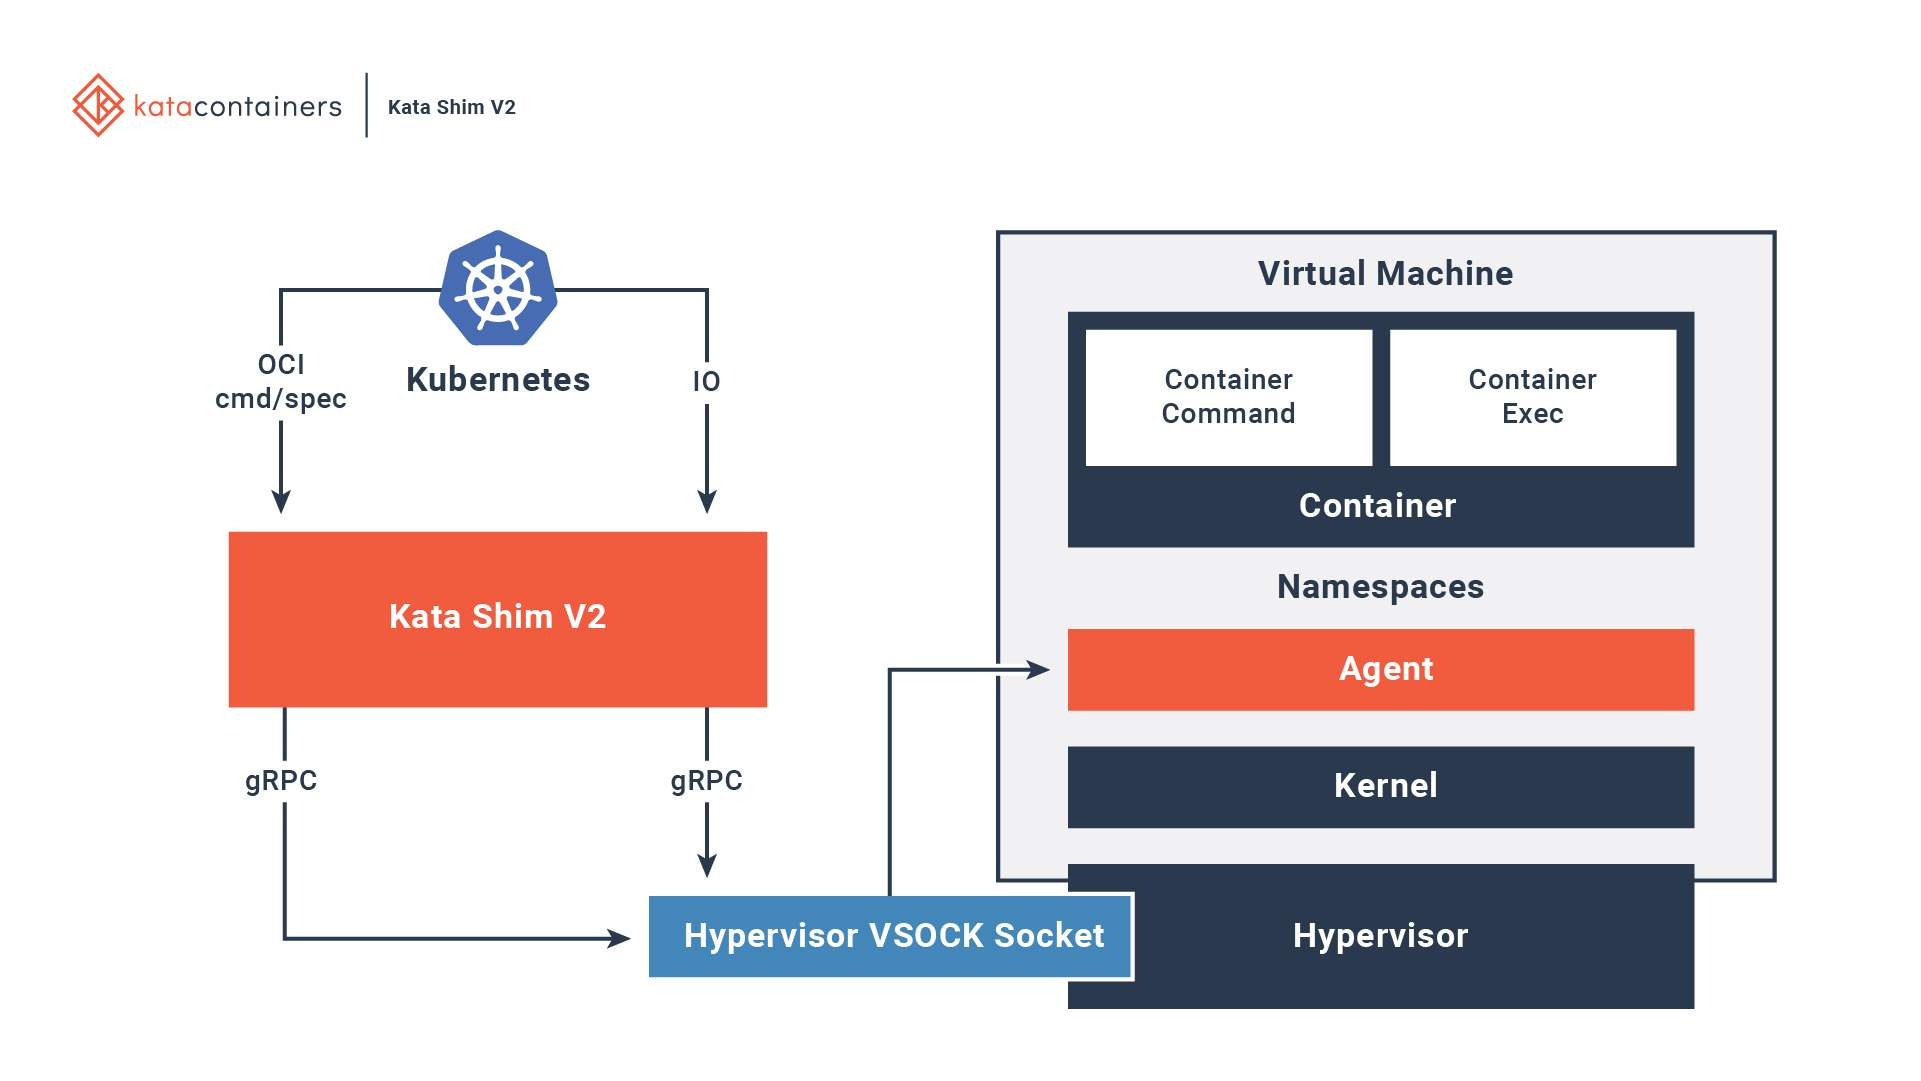
\includegraphics[width=13.5cm]{images/KataContainersArchitecture.jpg}
    \caption{Kata Containers 2.0 architecture \cite{KataContainers}}
    \label{fig:KataContainersArchitecture}
  \end{center}
\end{figure}

\begin{figure}[ht]
  \begin{center}
    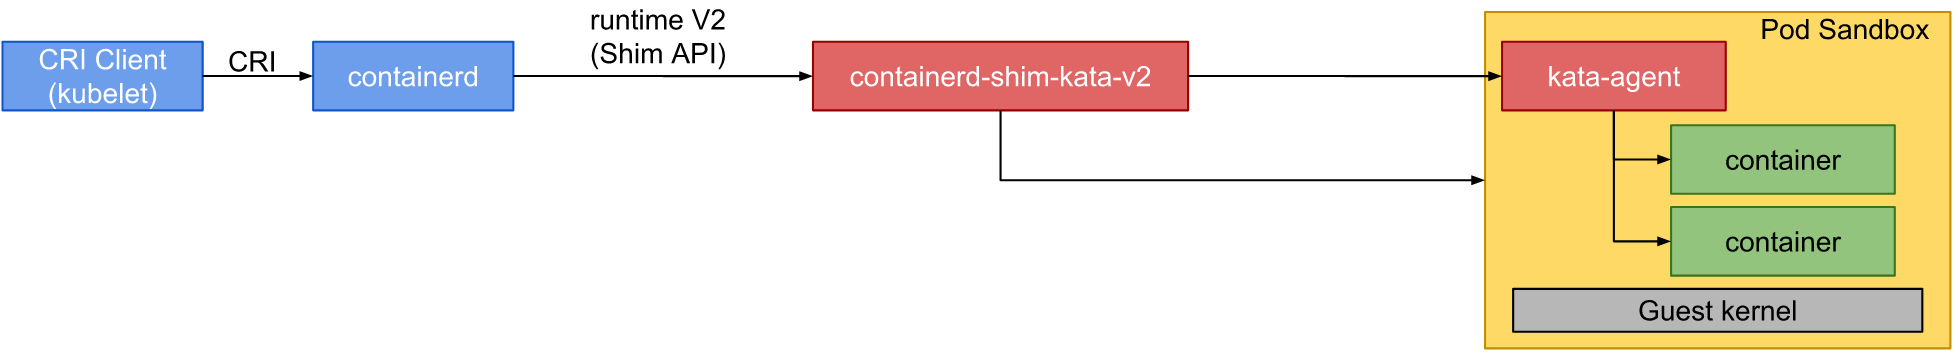
\includegraphics[width=13.5cm]{images/KataContainersComponents.png}
    \caption{Kata Containers 2.0 components \cite{KataContainersArchitecture}}
    \label{fig:KataContainersComponents}
  \end{center}
\end{figure}

\subsection{Kubernetes}

Kubernetes acts as an container-orchestration system for automating deployment, scaling, and management of containerized applications \cite{Kubernetes}. Kubernetes offers flexible configuration and it can installed inside a VM or on bare-metal. Like most distributed computing platforms, a Kubernetes cluster consists of at least one master node and multiple compute nodes. Each node runs a container runtime, such as Docker or containerd, along with an agent that communicates with the master.

Each container is launched as a pod. Pods are the atomic unit on the Kubernetes platform. A single node can include multiple pods inside it, and each pod is tied to the node it is created within. A runtime can be selected on a pod level, thus a single node can consists of workloads with various runtimes. This comes handy, whenever non-confidential, but highly performance-centric applications needs to be deployed in a node within more security oriented applications.

\subsection{Containerd}

Containers inside Kubernetes are managed via a container runtime. Containerd is an implementation of the Kubernetes CRI to enable using OCI compatible runtimes. It is an industry-standard container runtime with an emphasis on simplicity, robustness and portability. It is available as a daemon for Linux and Windows, which can manage the complete container lifecycle of its host system. The flexibility of containerd allows Kubernetes to register and use various OCI-compliant runtimes, such as Kata Containers, as container runtime for running pods. Containerd supports multiple means to download images including trust and image verification. Containerd also manages container process lifecycles, low-level storage, and resource isolation as required by the CRI. \cite{containerdGithub}\cite{containerd}

\subsection{Kata Shim V2}

The primary deliverable of the Kata Containers project is a CRI-friendly shim. The shim launches container runtime, which launches the container itself. The shim enables for daemonless containers, thus allowing runtime to exit after the container has been launched, and then becomes the parent of the container. \cite{Crosby}

\subsection{gRPC and ttRPC}

gRPC is a high performance Remote Procedure Call framework that can run in any environment. It connects services in and across data centers with pluggable support for load balancing, tracing, health checking and authentication. This protocol allows the runtime to send container management commands to the agent. The protocol is also used to carry the I/O streams such as stdout, stderr, and stdin, between the containers and manage the engine, which is containerd in this Thesis. \cite{gRPC}\cite{KataContainersArchitecture}

However, gRPC requires a lot of memory overhead for importing packages and at runtime. While this is great for many services with low density requirements, this can be a problem when running a large number of services on a single machine or on a machine with a small amount of memory. ttRPC also offers harnessed security by limiting attack surface and improved observability via metrics about the runtime itself, the VMM, as well as the guest kernel. Kata Shim V2 offers the support for ttRPC protocol to communicate with the agent. \cite{ttRPC}

\subsection{Hypervisor}

The VM of Kata Containers instance is launched by Virtual Machine Monitor (VMM). VMM consists of Virtual Machine Manager and a hypervisor. Kata Containers currently supports four different VMMs: ACRN hypervisor, Cloud Hypervisor, QEMU, and Firecracker. All these VMMs are open source projects.

ACRN is a reference hypervisor, which is built to meet the needs of embedded IoT development. It is developed with low overhead,fast boot-up, and configurations to support variety of devices and deployment scenarios. ACRN is a type 1 reference hypervisor stack that runs on bare-metal hardware, addressing the gap that currently exists between data center hypervisors, and hard partitioning hypervisors. \cite{ACRN}

Cloud Hypervisor is a VMM that runs on top of Kernel-based Virtual Machine (KVM). The project focuses on exclusively running modern, cloud workloads, on top of a limited set of hardware architectures and platforms. Cloud workloads refers to those that are usually run by customers inside a cloud provider, and most I/O are handled by performant para-virtualized devices, such as Virtio. \cite{CloudHypervisor}

QEMU is a generic machine, userspace emulator, and virtualizer. QEMU is capable of emulating a complete machine in software without any need for hardware virtualization support. It can also integrate with the Xen and KVM hypervisors to provide emulated hardware while allowing the hypervisor to manage the CPU. \cite{QEMUGithub}\cite{QEMU}

Firecracker VMM is developed by Amazon Web Services (AWS). Firecracker uses KVM to launch workload in lightweight micro virtual machines. Of Amazon's cloud products, Firecracker is deployed at least in AWS Lambda and Fargate. Firecracker currently supports Intel CPUs, with AMD and Arm support in developer preview. \cite{AWS}\cite{FirecrackerDesign}\cite{Debab2021}

\subsection{Agent}

Agent, also known as Kata-Agent, resides inside the Kubernetes pod in the computing node and its main task is to spawn the container process. The agent process runs as a daemon inside the virtual machine. This agent runs a ttRPC or gRPC server in the guest using a Virtio serial or VSOCK interface which the VMM exposes as a socket file on the host. \cite{KataContainersArchitecture}

\subsection{Container}

Container in Kata Containers architecture is isolated by wrapping it inside a dedicated kernel. This extra layer provides isolation of network. I/O and memory can utilize hardware-enforced isolation with virtualization VT extensions. Wrapping the container inside a micro VM adds a overhead to performance, which is discussed more in Chapter \ref{chapter:evaluation}. \cite{KataContainers}

Kata Containers is OCI compliant, thus the same standard shared by Docker containers guarantees compatibility. For now, only Linux operating systems and container images are supported in host and guest.

\section{Isolation and resource allocation}

In Kubernetes environment applications are deployed inside a pod. Whenever a new pod is created, it requests resources, which most commonly are CPU, memory, and huge pages, defined in the manifest. The allocated resources are reserved for the application running. Traditionally the resources allocated are a slice from the resource as described in the Figure \ref{fig:KataContainersStack}. In Kata Containers environment the hardware is virtualized for the guest kernel.

Kata Containers, a second layer of isolation is created on top of those provided by traditional namespace-containers. The hardware virtualization interface is the basis of this additional layer. Kata Containers launches a lightweight virtual machine, and uses the guest's Linux kernel to create a container workload. In Kubernetes and in the Kata implementation, the sandbox is carried out at the pod level. This sandbox is created using a virtual machine such as KVM. \cite{KataContainersVirtualization}

The additional layer of isolation allows untrusted workloads to be run in the same system without compromising other containers security. Container escapes \cite{CVE-2020-14386}\cite{CVE-2019-5736} have been a serious threat to system using traditional isolation mechanisms such as namespaces, cgroups, and seccomp.

\begin{figure}[ht]
  \begin{center}
    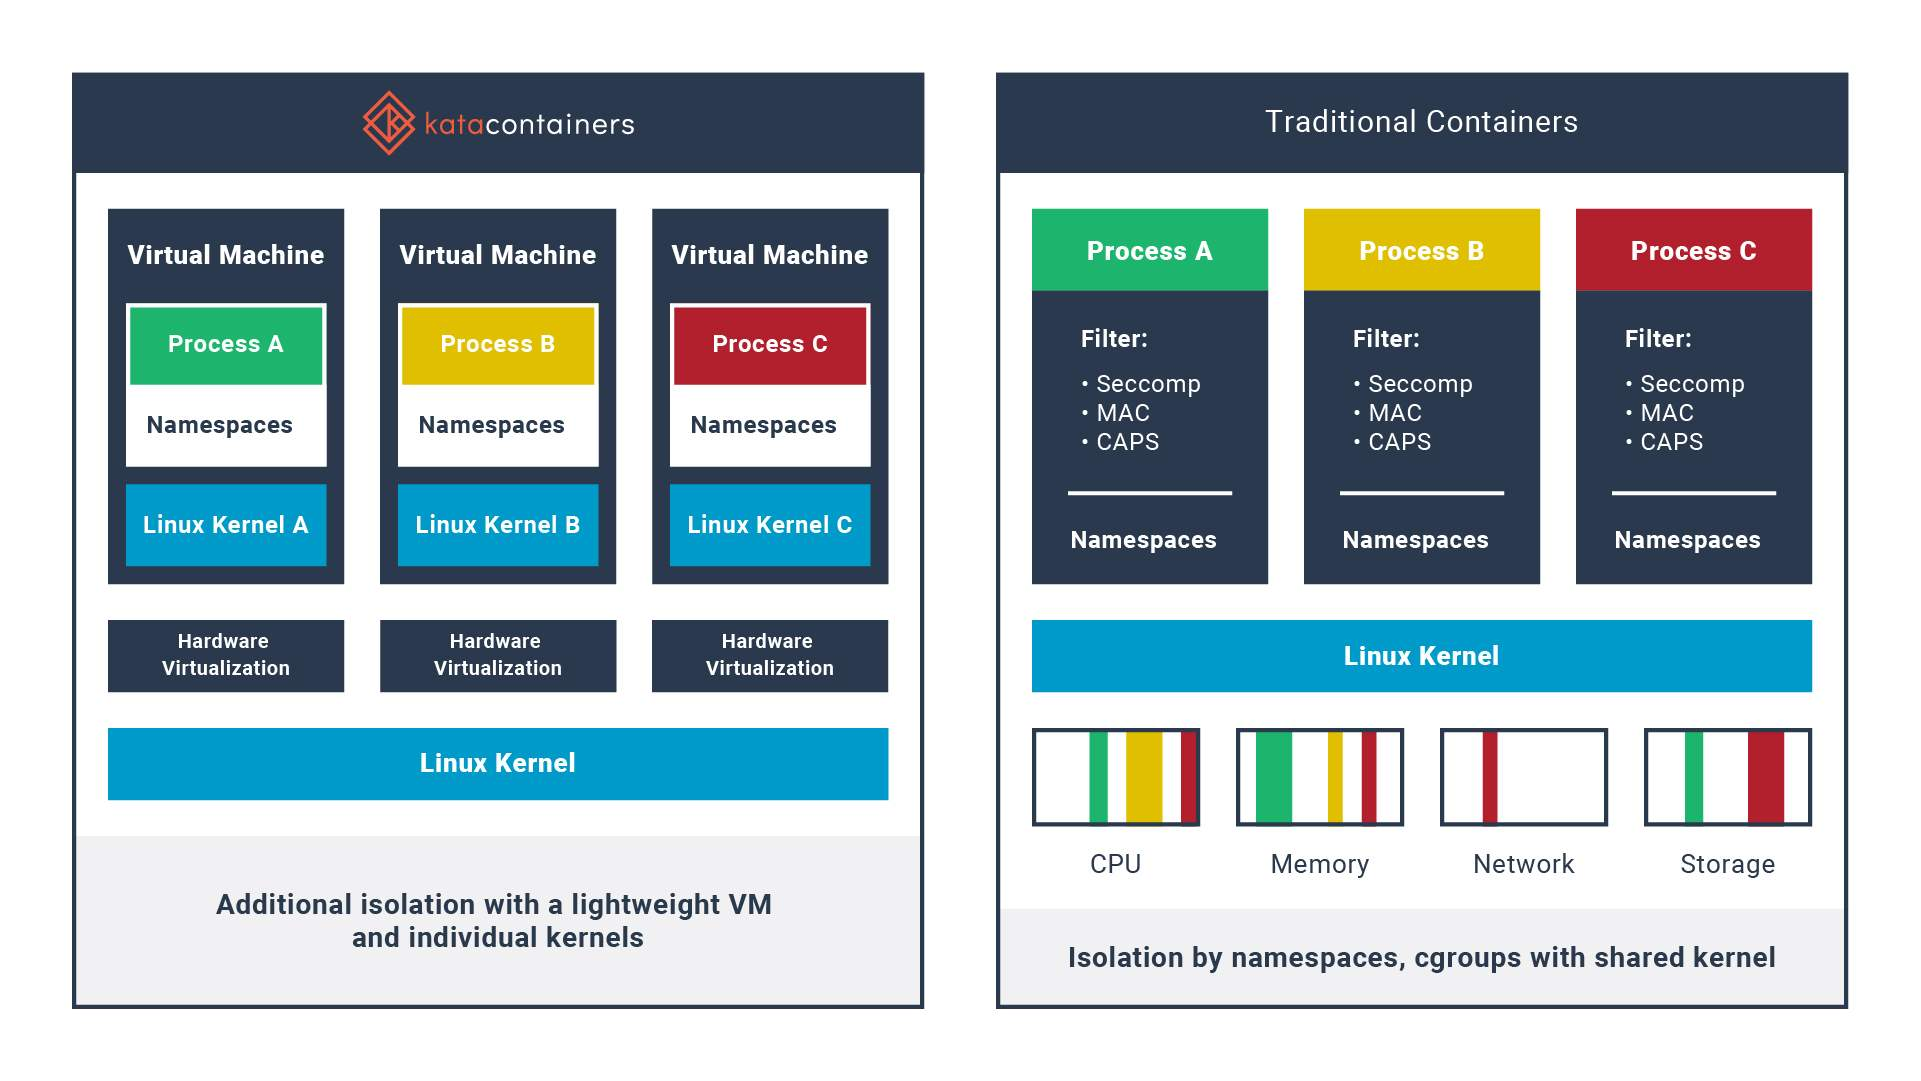
\includegraphics[width=13.5cm]{images/KataContainersStack.jpg}
    \caption{Kata Containers and traditional container stack \cite{KataContainers}}
    \label{fig:KataContainersStack}
  \end{center}
\end{figure} 

\section{Networking}

Traditionally container engines, such as Docker, add add one end of a virtual ethernet pair into the container networking namespace. The other end of the pair is added to the host networking namespace. However, many VMMs cannot handle the virtual ethernet interfaces. Typically, TAP interfaces are created for VM connectivity. Kata runtime overcomes the incompatibility between typical container engines expectations and virtual machines by connecting virtual ethernet interfaces with TAP ones using Traffic Control. The network is described in Figure \ref{fig:KataContainersNetwork}. \cite{KataContainersArchitecture}

Kata Containers runtime supports Container Network Interface (CNI) \cite{CNI} plugins, such as Calico, Weave, and SR-IOV. Both IPv4 and IPv6 networks are supported by the project.

\begin{figure}[ht]
  \begin{center}
    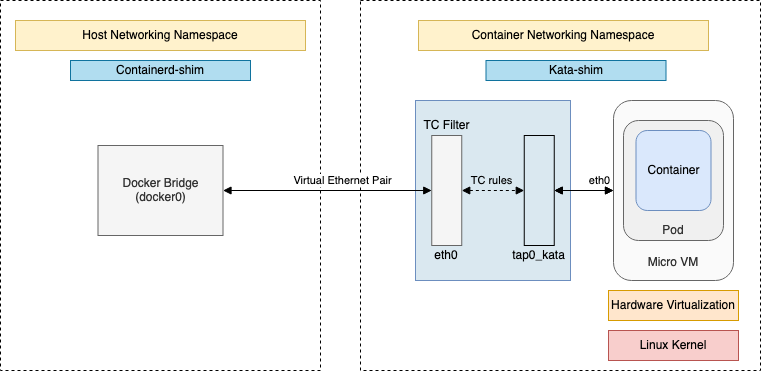
\includegraphics[width=13.5cm]{images/KataContainersNetwork.png}
    \caption{Kata Containers network overview \cite{KataContainersArchitecture}}
    \label{fig:KataContainersNetwork}
  \end{center}
\end{figure}

\section{Storage}

Container workloads are shared with the virtualized environment through virtio-fs. This shared file system that lets virtual machines access a directory tree on the host. In Kata Containers, virtio-fs can be used to share container volumes, secrets, config-maps, configuration files, and the container rootfs on the host with the guest. virtio-fs provides significant performance and POSIX compliance improvements compared to 9pfs. Virtio-fs was started at Red Hat and is being developed in the Linux, QEMU, FUSE, and Kata Containers open source communities. \cite{virtio-fs-Kata}\cite{virtio-fs}

Kata Containers has an ability to hot-plug and remove block devices, which is a data storage device that supports reading and optionally writing data in fixed-size blocks, sectors, or clusters. This support for hot-plugging makes it possible to use block devices for containers started after the VM has been launched. The support for hot-plug and file systems might vary depending on the VMM and hypervisor. \cite{KataContainersArchitecture}\cite{KataContainersVirtualization}

\section{Related work}

Kata Containers is not the sole option providing secure container runtime nor isolation in the container kernel layer. Microsoft offers a container instance isolation option inside Azure with Hyper-V. The hardware isolation is based on VMs, likewise in KC and Firecracker, thus leveraging the additional kernel layer. \cite{Hyper-V}

gVisor provides a second isolation method, differing from Kata Containers and Firecracker. gVisor intercepts application system calls and acts as the guest kernel without translating through virtualized hardware. The architecture can be thought of as a merged kernel and VMM. gVisor includes OCI runtime runsc, which provides the isolation boundary between the application and host kernel. Google develops gVisor, and it is harnessed in various Google's cloud products such as Kubernetes Engine \cite{GKE} and Cloud Run \cite{CloudRun}. \cite{Debab2021}\cite{gVisor}

A second approach for container isolation is IBM Nabla \cite{Nabla}. Nabla containers use library OS, also known as unikernel, to avoid system calls and reduce the attack surface. Nabla is based on a custom VMM named Nabla Tender to manage lightweight VMs executing unikernels. Nabla containers only use seven system calls, blocking all others via a Linux seccomp policy. The Nabla Tender intercepts hypercalls related to storage and network from unikernel VMs and translates them into syscalls to the host. \cite{Debab2021}

All the before-mentioned projects are open source and actively maintained. However, Nabla seems to be slightly less active in comparison to the other projects. Commercial and enterprise cloud platforms, such as AWS, uses Firecracker, and GKE uses gVisor. However, it is unknown for security reasons which approaches are used in the other platforms to isolate containers.


% that it fits to the same space as the text (total width = \textwidth).
% If you do need more space, you can either
% 1) ignore the LaTeX warnings 
% 2) use the textpos-package to manually position the table (read the package
%    documentation)
% 3) if you have the table as a PDF document (of correct size, A4), you can use
%    the pdfpages package to include the page. This overrides the margin
%    settings for this page and LaTeX will not complain.
% ------------------------------------------------------------------
% Another note:
% ------------------------------------------------------------------
% If your table fits to \textwidth, but the cells are so narrow that the text
% in p{..}-formatted cells does not flow nicely (you get underfull warnings 
% because LaTeX tries to justify the text in the cells) you can manually set
% the text to unjustified by using the \raggedright command for each cell 
% that you do not want to be justified (see the example below). \raggedleft 
% is also possible, of course...